\documentclass{beamer}

\title
{SIMT Branch Prediction}
\subtitle{Mitigating Stalls}
\author
{Steven Braeger \and Nick Arnold}
\institute
{
  \inst{1}%
  University of Central Florida
}
\date
{\today}

\begin{document}
\frame{\titlepage}

\begin{frame}
	\frametitle{Generic CPU Core Design}
	\begin{tabular}{c}
		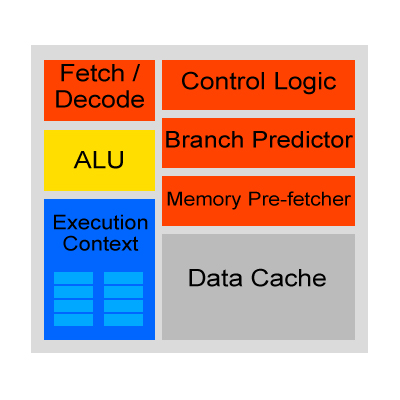
\includegraphics[width=.75\textwidth]{CPU-design.jpg}
	\end{tabular}
\end{frame}

\begin{frame}
	\frametitle{Generic CPU Core Design (cont.)}
	\begin{itemize}
		\item Regular Processor Logic
		\begin{itemize}
			\item Fetch/Decode Logic
			\item ALU for execution
			\item Execution Context (registers, etc.)
		\end{itemize}
		\item Single Thread Speedup Logic
		\begin{itemize}
			\item Control Logic
			\item Branch Predictor
			\item Memory Pre-fetcher
		\end{itemize}
		\item Data Cache
	\end{itemize}
\end{frame}

\begin{frame}
	\frametitle{Generic CPU Core Design (cont.)}
	\begin{itemize}
		\item What does this core do well?
		\begin{itemize}
			\item Single Instruction, Single Data (SISD)
			\begin{itemize}
				\item Control logic built to support this
			\end{itemize}
		\end{itemize}
		\item What does this core do poorly?
		\begin{itemize}
			\item Single Instruction, Multiple Data (SIMD)
			\item Multiple Instruction, Single Data (MISD)
			\item Miltiple Instruction, Multiple Data (MIMD)
		\end{itemize}
	\end{itemize}
\end{frame}

\begin{frame}
	\frametitle{Generic Multicore CPU Design}
	\begin{tabular}{c}
		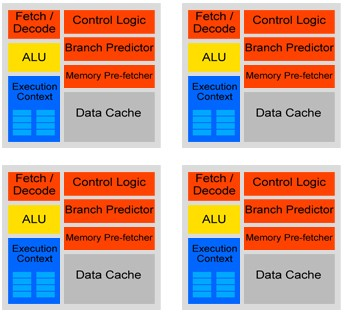
\includegraphics[width=.75\textwidth]{Multicore-CPU-design.jpg}
	\end{tabular}
\end{frame}

\begin{frame}
	\frametitle{Generic Multicore CPU Design (cont.)}
	\begin{itemize}
		\item What does this core do well?
		\begin{itemize}
			\item SISD
			\begin{itemize}
				\item Multiple independent processes
				\item Idling
			\end{itemize}
			\item MISD
			\begin{itemize}
				\item Independent instructions from one process (out of order)
			\end{itemize}
		\end{itemize}
		\item What does this core do poorly?
		\begin{itemize}
			\item SIMD
			\item MIMD
		\end{itemize}
	\end{itemize}
\end{frame}

\begin{frame}
	\frametitle{Generic GPU Core Design}
	\begin{tabular}{c}
		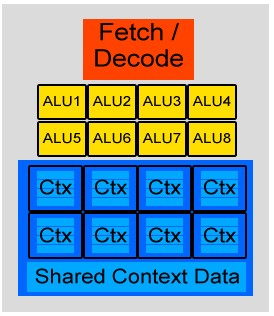
\includegraphics[width=.75\textwidth]{GPU-Design.jpg}
	\end{tabular}
\end{frame}

\begin{frame}
	\frametitle{Generic GPU Core Design (cont.)}
	\begin{itemize}
		\item What's different?
		\begin{itemize}
			\item Removed single threading speedup logic
			\item Removed data cache
			\item Added multiple execution contexts
		\end{itemize}
		\item Why do this?
		\begin{itemize}
			\item Designed for graphics processing
			\item Tailored specifically to those types of instruction streams
			\item Performing the same operations on many independent data elements
		\end{itemize}
	\end{itemize}
\end{frame}

\begin{frame}
	\frametitle{Generic GPU Core Design (cont.)}
	\begin{itemize}
		\item What does this core do well?
		\begin{itemize}
			\item SIMD
			\begin{itemize}
				\item Similar contexts assigned to GPU
				\item Core performs the same computations on all contexts
			\end{itemize}
		\end{itemize}
		\item What does this core do poorly?
		\begin{itemize}
			\item SISD
			\item MISD
			\item MIMD
		\end{itemize}
	\end{itemize}
\end{frame}

\begin{frame}
	\frametitle{Generic GPU Core Design (cont.)}
	\begin{tabular}{c}
		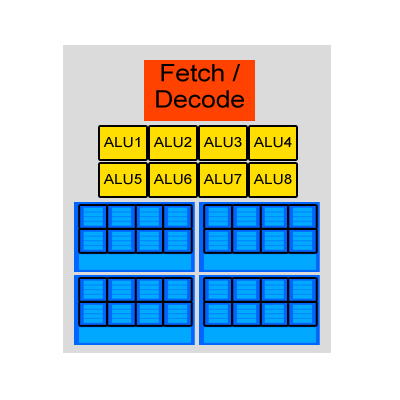
\includegraphics[width=.75\textwidth]{GPU-Design---multiple-contexts.jpg}
	\end{tabular}
\end{frame}

\begin{frame}
	\frametitle{Generic GPU Core Design (cont.)}
	\begin{itemize}
		\item GPUs can modify their context storage 
		\item Separate into various smaller contexts
		\item Try and hide stalls (more on this later)
	\end{itemize}
\end{frame}

\begin{frame}
	\frametitle{Generic Multicore GPU Design}
	\begin{tabular}{c}
		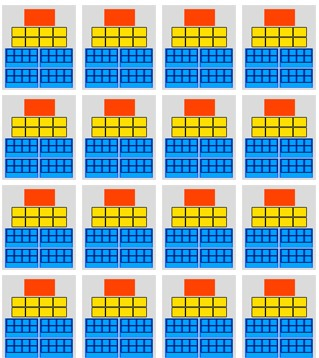
\includegraphics[width=.75\textwidth]{GPU-Design---multiple-cores.jpg}
	\end{tabular}
\end{frame}

\begin{frame}
	\frametitle{Generic Multicore GPU Design (cont.)}
	\begin{itemize}
		\item What does this core do well?
		\begin{itemize}
			\item SIMD
			\begin{itemize}
				\item All cores assigned same instruction stream
			\end{itemize}
			\item MIMD
			\begin{itemize}
				\item Multiple independent tasks (vertices, fragments, etc.)
			\end{itemize}
		\end{itemize}
		\item What does this core do poorly?
		\begin{itemize}
			\item SISD
			\item MISD
		\end{itemize}
	\end{itemize}
\end{frame}

\begin{frame}
	\frametitle{GPU Context Interleaving}
	\begin{tabular}{c}
		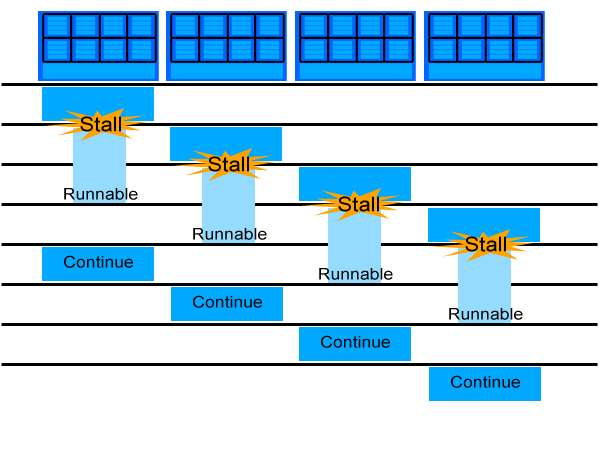
\includegraphics[width=.75\textwidth]{GPU-context-interleaving.jpg}
	\end{tabular}
\end{frame}

\begin{frame}
	\frametitle{GPU Context Interleaving (cont.)}
	\begin{itemize}
		\item GPU is always utilizing ALUs optimally, even though contexts are waiting
		\item If wait time exceeds certain amount, the GPU must stall
	\end{itemize}
\end{frame}

\begin{frame}
	\frametitle{GPU Context Interleaving (cont.)}
	\begin{tabular}{c}
		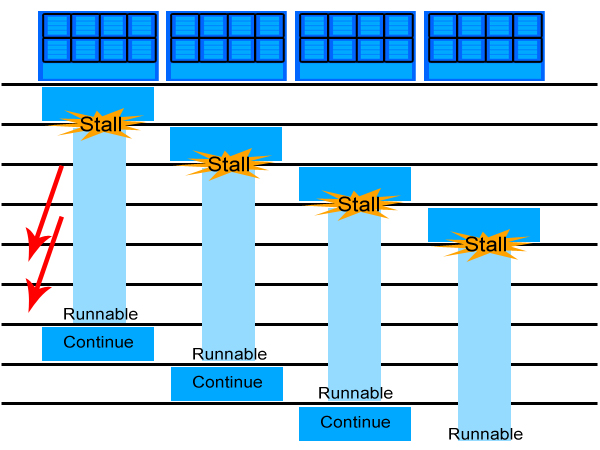
\includegraphics[width=.75\textwidth]{GPU-context-interleaving-2.jpg}
	\end{tabular}
	\begin{itemize}
		\item Red arrows indicate idle cycles due to stalling for 1st context group's branch
		\item What if we could avoid this?
	\end{itemize}
\end{frame}

\begin{frame}
	\frametitle{Branch Prediction on CPU}
	\begin{itemize}
		\item On CPUs, each core has one execution context and one branch prediction table
		\item Each context handles its own predictions
		\begin{itemize}
			\item No assistance from other threads 
			\item No way to guarantee what the other threads are doing
		\end{itemize}
		\item On GPUs, each core has multiple execution contexts
		\begin{itemize}
			\item All contexts assigned to that core are performing the same operations
			\item Couldn't we use this information to assist other contexts?
		\end{itemize}
	\end{itemize}
\end{frame}

\begin{frame}
	\frametitle{GPU Programs}
	\begin{itemize}
		\item GPUs bundle several contexts together into context groups
		\item Collection of all contexts belonging to one GPU core is a 'warp'
		\item All contexts within a warp will be subjected to the same instruction stream
		\begin{itemize}
			\item Processed context group by context group
			\item High degree of spatial locality
		\end{itemize}
		\item Take advantage of information discovered by the first context group 
	\end{itemize}
\end{frame}

\begin{frame}
	\frametitle{Our Proposal}
	\begin{itemize}
		\item Introduce 3 GPU Branch Predictors with the following features
		\begin{itemize}
			\item One predictor is shared amongst the contexts within a GPU
			\item One predictor is shared only amongst its context group (1 per group)
			\item One predictor is shared only amongst its context (1 per context)
		\end{itemize}
		\item Predictor table is the size of the instruction stream to avoid collisions
		\begin{itemize}
			\item Types of instruction streams that are issued to GPUs are by their nature not very long
		\end{itemize}
		\item Predictor table entries are Smith 2-bit predictors
		\item Compare prediction accuracies across these implementations
	\end{itemize}
\end{frame}

\begin{frame}
	\frametitle{Our Proposal (cont.)}
	\begin{tabular}{c}
		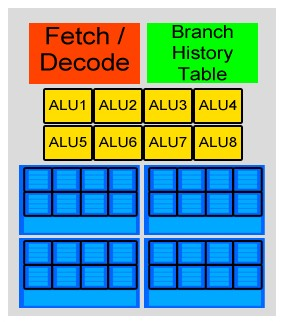
\includegraphics[width=.5\textwidth]{Our-GPU---per-core-predictor.jpg}
	\end{tabular}
\end{frame}

\begin{frame}
	\frametitle{Our Proposal (cont.)}
	\begin{tabular}{c}
		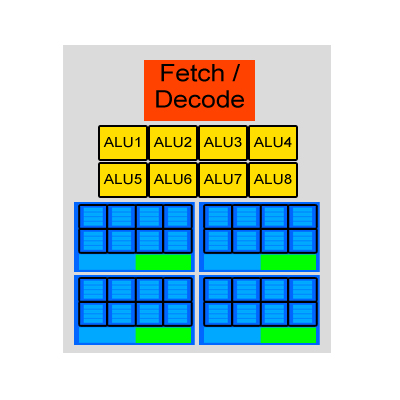
\includegraphics[width=.5\textwidth]{Our-GPU---per-context-group-predictor.jpg}
	\end{tabular}
\end{frame}

\begin{frame}
	\frametitle{Our Proposal (cont.)}
	\begin{tabular}{c}
		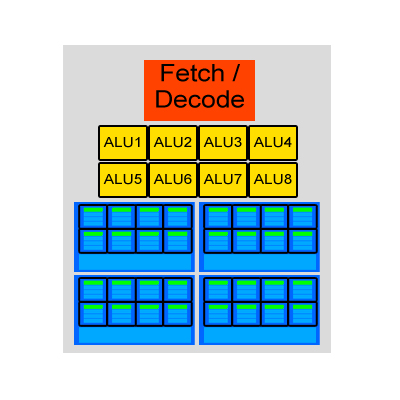
\includegraphics[width=.5\textwidth]{Our-GPU---per-element-predictor.jpg}
	\end{tabular}
	\begin{itemize}
		\item This implementation most closely resembles how a regular CPU core handles branch prediction
	\end{itemize}
\end{frame}

\begin{frame}
    \frametitle{Branch Predictor}
    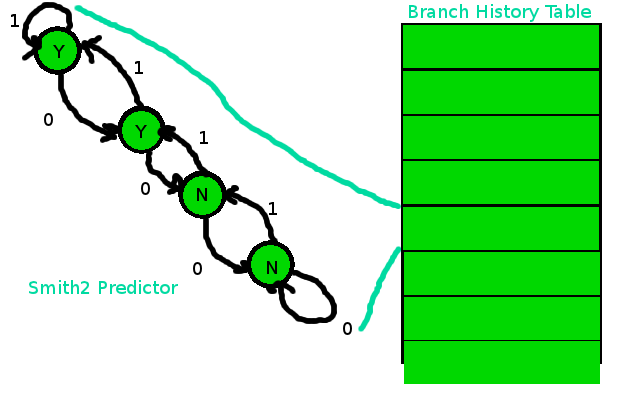
\includegraphics[height=.6\textheight]{bht.png}
    \begin{itemize}
     \item Limited Kernel Size.  Max 16k instructions.
     \item 16k BHT entries==no collisions.  4KiB of memory.
    \end{itemize}
\end{frame}


\begin{frame}
	\frametitle{Our Proposal (cont.)}
	\begin{tabular}{c}
		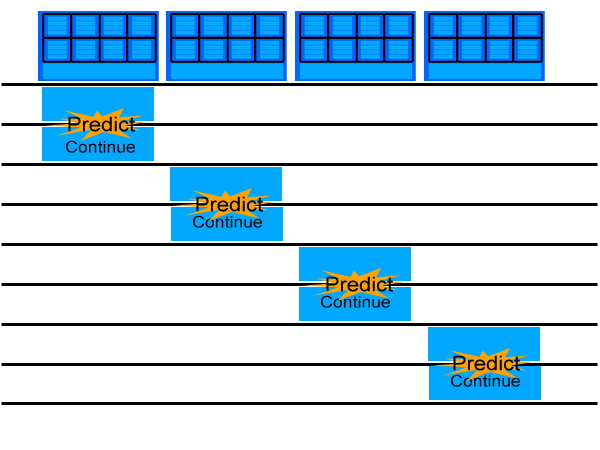
\includegraphics[width=.75\textwidth]{GPU-predict-context.jpg}
	\end{tabular}
\end{frame}

\begin{frame}
   \frametitle{Experiment}
   \begin{itemize}
    \item Must have appropriate simulator modeling SIMT architecture.
    \item SimpleScalar NOT sufficient
    \item GPGPU-Sim: Rewrite based on SimpleScalar.
    \item Simulates an NVIDIA Quadro 5800. (16k register file, 4 GB ram, 32 cores,1024 contexts)
    \item Creates libcuda.so and libOpenCL.so to intercept GPU commands from CPU program.
    \item Requires NVIDIA hardware (driver does compilation) to build benchmarks.
   \end{itemize}
\end{frame}

\begin{frame}
 \frametitle{Simulation Architecture (slide courtesy of gpgpu)}
  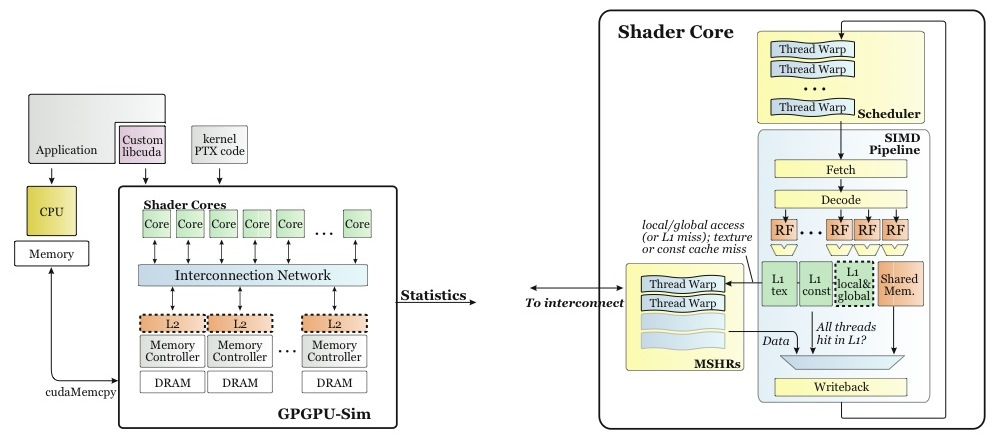
\includegraphics[width=.9\textwidth]{uarch.jpg}

\end{frame}

\begin{frame}
 \frametitle{Benchmarks (ISPASS09)}
 \begin{itemize}
  \item Subset of ISPASS09 CUDA benchmarks
  \item Some benchmarks failed
  \item Run for 4 days
  \item CPU component failed to meet dependencies
  \item CUDA Architecture unsupported (double/single)
  \item No branching!  (AES)
 \end{itemize}
\end{frame}

\begin{frame}
 \frametitle{ISPASS09 Benchmarks (cont.)}
\begin{itemize}
 \item \emph{NQU} Solve the NQUEENS problem
 \item \emph{NN} Classify images with a neural net
  \item \emph{RAY} Raytrace a scene
\item \emph{BFS} Breadth-First Search a graph.
\end{itemize}
\end{frame}

\begin{frame}
\frametitle{Results}
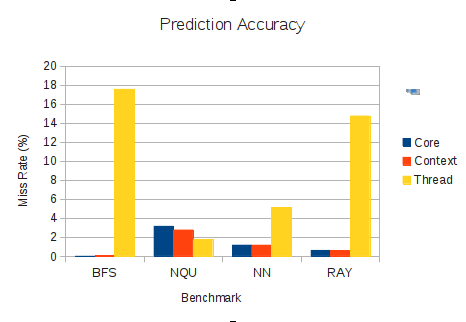
\includegraphics[width=.9\textwidth]{data.png}
\end{frame}

\begin{frame}
 \frametitle{Results (cont.)}
\begin{itemize}
 \item Significant improvement over per-thread predictor
 \item NQUEENS failed...DP solution mispredicts parallel neighbors?
\end{itemize}

\end{frame}

\begin{frame}
 \frametitle{Any Questions?}
\begin{itemize}
 \item Question: 
\end{itemize}

\end{frame}








\end{document}

